% \IUref{IUAdmPS}{Administrar Planta de Selección}
% \IUref{IUModPS}{Modificar Planta de Selección}
% \IUref{IUEliPS}{Eliminar Planta de Selección}

%\begin{UseCase}[archivo de imágen]{UCX}{Nombre del Caso de uso}{
	\begin{UseCase}{CU7.0}{Registrar áreas}{
		En esta sección el administrador podrá dar de alta una nueva área.
	}
		\UCitem{Versión}{1.0}
		\UCitem{Actor}{Gerente}
		\UCitem{Propósito}{Que se agreguen nuevas áreas para realizar alguna actividad.}
		\UCitem{Entradas}{Nombre del Área, Tipo de área, largo, ancho, capacidad, responsable y 					     descripción.}
		\UCitem{Origen}{Los datos serán digitados desde el teclado.}
		\UCitem{Salidas}{Mensaje de registro exitoso.}
		\UCitem{Destino}{Los datos serán enviados y almacenados en la base de datos, que 					contendrán ese nuevo registro.}
		\UCitem{Precondiciones}{Que no esté esa área registrada previamente.
		Que exista alguna actividad que pueda utilizar dicha área.}
		\UCitem{Postcondiciones}{El área registrada se verá reflejada en la sección de consultas.}
		\UCitem{Errores}{Que la información registrada no corresponda a los tipos de datos esperados.}
		\UCitem{Tipo}{Caso de uso primario}
		\UCitem{Observaciones}{}
		\UCitem{Autor}{Francisco García Enríquez.}
		\UCitem{Revisor}{Martin Carrillo.}
	\end{UseCase}


	\begin{UCtrayectoria}{Principal}
		\UCpaso[\UCactor] Selecciona del menú principal la opción Áreas.
		\UCpaso Muestra las opciones que el gerente pueda realizar: Registrar Áreas, Consultar Áreas, Eliminar Áreas, Dar de Baja Áreas y Actualizar Áreas.
		\UCpaso[\UCactor] Selecciona la opción de registrar áreas.
		\UCpaso Mostrará el formulario para registrar un área.		
		\UCpaso[\UCactor] Ingresará el nombre del área.
		\UCpaso[\UCactor] Confirma el registro presionando el botón de registrar.
		\UCpaso Muestra el mensaje {\bf MSG1-}``largo, ancho y responsable deben ser ingresados.'' 	
		\UCpaso[\UCactor] Ingresa caracteres en el campo largo y confirma el envio.
		\UCpaso Muestra un mensaje {\bf MSG2-}``campo largo debe ser numérico''
		\UCpaso Se queda en el campo largo para ingresar el dato correcto.
		\UCpaso[\UCactor] Confirma el registro y presiona el botón registrar.
		\UCpaso Manda un mensaje de error {\bf MSG3-}``el campo ancho debe ser ingresado''.
		\UCpaso devuelve el focus al campo ancho para corregir el dato.
		\UCpaso[\UCactor] Ingresa en el campo ancho un carácter como registro.
		\UCpaso[\UCactor] Confirma el registro presionando el botón registrar.
		\UCpaso Le manda un mensaje de error, {\bf MSG4-}``campo ancho debe ser numérico''.
		\UCpaso[\UCactor] Ingresa un dato numérico en el campo ancho.
		\UCpaso[\UCactor] Confirma el registro presionando el botón  de registrar área.
		\UCpaso Le manda un mensaje de error, {\bf MSG5-}``el campo responsable debe ser ingresado''.
		\UCpaso[\UCactor] Ingresa un dato numérico en el campo responsable.
		\UCpaso le manda un mensaje de error, {\bf MSG6-}``el campo responsable solo acepta letras y espacios en blanco''. 
		\UCpaso[\UCactor] Ingresa letras y espacios en blanco en el campo responsable.
		\UCpaso[\UCactor] Confirma el registro, presionando el botón de registrar área.
		\UCpaso Muestra una pantalla con un mensaje, {\bf MSG7-}``el registro fue exitoso''.
	\end{UCtrayectoria}
		
		\begin{UCtrayectoriaA}{A}{El gerente no llena la información con el tipo de dato correspondiente.}
			\UCpaso[\UCactor] Introduce espacios en blanco al inicio o caracteres especiales asi como datos numericos en el campo nombre.
			\UCpaso[\UCactor] Confirma el registro y presiona el boton registrar.
			\UCpaso Mostrará un mensaje  {\bf MSG8-}``el campo solo acepta letras y espacios en blanco''.
			\UCpaso[] Termina el caso de uso.
		\end{UCtrayectoriaA}

\begin{figure}[htbp!]
		\centering
			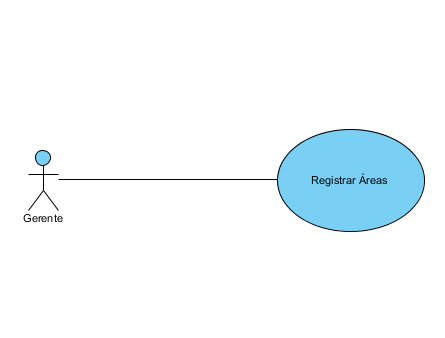
\includegraphics[width=0.8\textwidth]{images/ResgistraArea}
		\caption{Diagrama de Casos de Uso del sistema.}
	\end{figure}